\documentclass[a4paper, 12pt]{report}		% general format

%%%% Charset
\usepackage{cmap}							% make PDF files searchable and copyable
\usepackage[utf8]{inputenc}					% accept different input encodings
\usepackage[T2A]{fontenc}					% russian font
\usepackage[russian]{babel}					% multilingual support (T2A)

%%%% Graphics
\usepackage[dvipsnames]{xcolor}			% driver-independent color extensions
\usepackage{graphicx}						% enhanced support for graphics
\usepackage{wrapfig}						% pro­duces fig­ures which text can flow around

%%%% Math
\usepackage{amsmath}						% Amer­i­can Math­e­mat­i­cal So­ci­ety (AMS) math fa­cil­i­ties
\usepackage{amsfonts}						% fonts from the AMS
\usepackage{amssymb}						% additional math symbols

%%%% Ty­po­grapy (don't forget about cm-super)
\usepackage{microtype}						% sublim­i­nal re­fine­ments to­wards ty­po­graph­i­cal per­fec­tion
\linespread{1.3}							% line spacing
\usepackage[left=2.5cm, right=1.5cm, top=2.5cm, bottom=2.5cm]{geometry}
\setlength{\parindent}{0pt}					% we don't want any paragraph indentation
\usepackage{parskip}						% add distance between paragraphs
\renewcommand{\chaptername}{}

%%%% Other
\usepackage{url}							% ver­ba­tim with URL-sen­si­tive line breaks
%\DeclareUnicodeCharacter{00A0}{~}

%------------------------------------------------------------------------------
\usepackage{listings}						% type­set source code list­ings

% Цвета для кода
\definecolor{string}{HTML}{101AF9}			% цвет строк в коде
\definecolor{comment}{HTML}{3F7F5F}		% цвет комментариев в коде
\definecolor{keyword}{HTML}{5F1441}		% цвет ключевых слов в коде
\definecolor{morecomment}{HTML}{8000FF}	% цвет include и других элементов в коде
\definecolor{captiontext}{HTML}{FFFFFF}	% цвет текста заголовка в коде
\definecolor{captionbk}{HTML}{999999}		% цвет фона заголовка в коде
\definecolor{bk}{HTML}{FFFFFF}				% цвет фона в коде
\definecolor{frame}{HTML}{999999}			% цвет рамки в коде

% Настройки отображения кода
\lstset{
	language=C++,							% Язык кода по умолчанию
	morekeywords={*,...},					% если хотите добавить ключевые слова, то добавляйте
	% Цвета
	keywordstyle=\color{keyword}\ttfamily\bfseries,
	stringstyle=\color{string}\ttfamily,
	commentstyle=\color{comment}\ttfamily\itshape,
	morecomment=[l][\color{morecomment}]{\#},
	% Настройки отображения
	breaklines=true,						% Перенос длинных строк
	basicstyle=\ttfamily\footnotesize,		% Шрифт для отображения кода
	backgroundcolor=\color{bk},				% Цвет фона кода
	%frame=lrb,xleftmargin=\fboxsep,xrightmargin=-\fboxsep, % Рамка, подогнанная к заголовку
	frame=tblr								% draw a frame at all sides of the code block
	rulecolor=\color{frame},				% Цвет рамки
	tabsize=2,								% tab space width
	showstringspaces=false,					% don't mark spaces in strings
	% Настройка отображения номеров строк. Если не нужно, то удалите весь блок
	numbers=left,							% Слева отображаются номера строк
	stepnumber=1,							% Каждую строку нумеровать
	numbersep=5pt,							% Отступ от кода
	numberstyle=\small\color{black},		% Стиль написания номеров строк
	% Для отображения русского языка
	extendedchars=true,
	literate={Ö}{{\"O}}1
	 	{Ä}{{\"A}}1
	 	{Ü}{{\"U}}1
		{ß}{{\ss}}1
		{ü}{{\"u}}1
		{ä}{{\"a}}1
		{ö}{{\"o}}1
		{~}{{\textasciitilde}}1
		{а}{{\selectfont\char224}}1
		{б}{{\selectfont\char225}}1
		{в}{{\selectfont\char226}}1
		{г}{{\selectfont\char227}}1
		{д}{{\selectfont\char228}}1
		{е}{{\selectfont\char229}}1
		{ё}{{\"e}}1
		{ж}{{\selectfont\char230}}1
		{з}{{\selectfont\char231}}1
		{и}{{\selectfont\char232}}1
		{й}{{\selectfont\char233}}1
		{к}{{\selectfont\char234}}1
		{л}{{\selectfont\char235}}1
		{м}{{\selectfont\char236}}1
		{н}{{\selectfont\char237}}1
		{о}{{\selectfont\char238}}1
		{п}{{\selectfont\char239}}1
		{р}{{\selectfont\char240}}1
		{с}{{\selectfont\char241}}1
		{т}{{\selectfont\char242}}1
		{у}{{\selectfont\char243}}1
		{ф}{{\selectfont\char244}}1
		{х}{{\selectfont\char245}}1
		{ц}{{\selectfont\char246}}1
		{ч}{{\selectfont\char247}}1
		{ш}{{\selectfont\char248}}1
		{щ}{{\selectfont\char249}}1
		{ъ}{{\selectfont\char250}}1
		{ы}{{\selectfont\char251}}1
		{ь}{{\selectfont\char252}}1
		{э}{{\selectfont\char253}}1
		{ю}{{\selectfont\char254}}1
		{я}{{\selectfont\char255}}1
		{А}{{\selectfont\char192}}1
		{Б}{{\selectfont\char193}}1
		{В}{{\selectfont\char194}}1
		{Г}{{\selectfont\char195}}1
		{Д}{{\selectfont\char196}}1
		{Е}{{\selectfont\char197}}1
		{Ё}{{\"E}}1
		{Ж}{{\selectfont\char198}}1
		{З}{{\selectfont\char199}}1
		{И}{{\selectfont\char200}}1
		{Й}{{\selectfont\char201}}1
		{К}{{\selectfont\char202}}1
		{Л}{{\selectfont\char203}}1
		{М}{{\selectfont\char204}}1
		{Н}{{\selectfont\char205}}1
		{О}{{\selectfont\char206}}1
		{П}{{\selectfont\char207}}1
		{Р}{{\selectfont\char208}}1
		{С}{{\selectfont\char209}}1
		{Т}{{\selectfont\char210}}1
		{У}{{\selectfont\char211}}1
		{Ф}{{\selectfont\char212}}1
		{Х}{{\selectfont\char213}}1
		{Ц}{{\selectfont\char214}}1
		{Ч}{{\selectfont\char215}}1
		{Ш}{{\selectfont\char216}}1
		{Щ}{{\selectfont\char217}}1
		{Ъ}{{\selectfont\char218}}1
		{Ы}{{\selectfont\char219}}1
		{Ь}{{\selectfont\char220}}1
		{Э}{{\selectfont\char221}}1
		{Ю}{{\selectfont\char222}}1
		{Я}{{\selectfont\char223}}1
		{і}{{\selectfont\char105}}1
		{ї}{{\selectfont\char168}}1
		{є}{{\selectfont\char185}}1
		{ґ}{{\selectfont\char160}}1
		{І}{{\selectfont\char73}}1
		{Ї}{{\selectfont\char136}}1
		{Є}{{\selectfont\char153}}1
		{Ґ}{{\selectfont\char128}}1
}

% Для настройки заголовка кода
\usepackage{caption}
\DeclareCaptionFont{white}{\color{сaptiontext}}
\DeclareCaptionFormat{listing}{\parbox{\linewidth}{\colorbox{сaptionbk}{\parbox{\linewidth}{#1#2#3}}\vskip-4pt}}
%\captionsetup[lstlisting]{format=listing,labelfont=white,textfont=white}
\renewcommand{\lstlistingname}{Листинг} % Переименование Listings в нужное именование структуры

%------------------------------------------------------------------------------
\begin{document}

\begin{titlepage}
\thispagestyle{empty}

\begin{center}
Санкт-Петербургский государственный политехнический университет \\
Институт Информационных Технологий и Управления \\*
Кафедра компьютерных систем и программных технологий \\*
\hrulefill
\end{center}

\vspace{18em}

\begin{center}
\Large Отчет по расчетной работе № 1 \\ по предмету «Системное программное обеспечение» \\
\end{center}

\vspace{1em}

% \linebreak
\begin{center}
\textsc{\textbf{Обработка исключений в ОС Windows}}
\end{center}

\vspace{16em}

\begin{flushleft}
Работу выполнил студент гр. 53501/3\hrulefill Мартынов С. А. \\
\vspace{1.5em}
Работу принял преподаватель \hrulefill Душутина Е. В. \\
\end{flushleft}

\vspace{\fill}

\begin{center}
Санкт-Петербург \\
2014
\end{center}

\end{titlepage}
%------------------------------------------------
\setcounter{page}{2}
\tableofcontents
%------------------------------------------------

\chapter*{Постановка задачи}
\addcontentsline{toc}{chapter}{Постановка задачи}

\begin{enumerate}
	\item Сгенерировать и обработать исключения с помощью функций WinAPI;
	\item Получить код исключения с помощью функции GetExceptionCode.
		\begin{itemize}
		\item Использовать эту функции в выражении фильтре;
		\item Использовать эту функцию в обработчике.
		\end{itemize}
	\item Создать собственную функцию-фильтр;
	\item Получить информацию об исключении с помощью функции GetExceptionInformation; сгенерировать исключение с помощью функции RaiseException;
	\item Использовать функции UnhandledExceptionFilter и SetUnhandledExceptionFilter для необработанных исключений;
	\item Обработать вложенные исключения;
	\item Выйти из блока \_\_try с помощью оператора goto;
	\item Выйти из блока \_\_try с помощью оператора \_\_leave;
	\item Преобразовать структурное исключение в исключение языка С, используя функцию translator;
	\item Использовать финальный обработчик finally;
	\item Проверить корректность выхода из блока \_\_try с помощью функции AbnormalTermination в финальном обработчике \_\_finally.
\end{enumerate}

На каждый пункт представить отдельную программу, специфический код, связанный с особенностями генерации заданного исключения структурировать в отдельный элемент (функцию, макрос или иное).

%------------------------------------------------

\chapter*{Введение}
\addcontentsline{toc}{chapter}{Введение}

Во время выполнения программы могут возникать ситуации, когда состояние внешних данных, устройств ввода-вывода или компьютерной системы в целом делает дальнейшие вычисления в соответствии с базовым алгоритмом невозможными или бессмысленными. В отсутствие собственного механизма обработки исключений для прикладных программ наиболее общей реакцией на любую исключительную ситуацию является немедленное прекращение выполнения с выдачей пользователю сообщения о характере исключения. Можно сказать, что в подобных случаях единственным и универсальным обработчиком исключений становится операционная система.

В операционной системе Microsoft Windows, механизм обработки программных и аппаратных исключений является SEH (Structured Exception Handling), позволяющий программистам контролировать обработку исключений, а также являющийся отладочным средством.

\vspace{1em}
В данной работе рассматриваются следующие исключения:
\begin{itemize}
\item \textbf{EXCEPTION\_FLT\_DIVIDE\_BY\_ZERO} - поток попытался сделать деление на ноль с плавающей точкой;
\item \textbf{EXCEPTION\_FLT\_OVERFLOW} - переполнение при операции над числами с плавающей точкой.
\end{itemize}

Для исследования результатов работы программы будет использоваться тройная система логгирования:
\begin{itemize}
\item вывод результатов работы на стандартное устройство вывода (как правило, это экран пользователя, но можно переопределить вывод в файл или на принтер);
\item запись протокола работы программы в лог-файл (все лог-файлы находятся в каталоге logs, некоторые приведены по ходу отчёта);
\item фиксирование события в системном журнале Windows, который является стандартным способом централизованного хранения информации о важных программных и аппаратных событиях (о работе с системным журналом будет рассказано подробнее в одной из задач).
\end{itemize}

Каждое событие может быть выгружено из журнала в виде файла. Для этого доступны следующие форматы:
\begin{itemize}
\item EVTX (Windows Event Log) -- это бинарный файл специфичной структуры;
\item XML -- форматированный текст;
\item TXT -- текстовый формат где значения полей разделены символом табуляции;
\item CSV -- текстовый формат где значения полей разделены запятой.
\end{itemize}

Журналы событий представляют собой особые файлы, в которые заносятся сведения о значимых событиях компьютера, например о входе пользователя в систему или об ошибках в приложениях. При возникновении подобных ошибок Windows их регистрирует в соответствующем журнале, который можно прочитать в окне просмотра событий. Сведения в журналах событий могут быть весьма полезны опытным пользователям для устранения неполадок в Windows и других программах.

Для доступа к просмотру событий журнала требуется нажать кнопку "Пуск", выбрать "Панель управления", "Система и безопасность", "Администрирование", затем дважды щелкнуть "Просмотр событий" (окно просмотра событий показано на рисунке 1).‌ Выбрать интересующий журнал событий можно в левой панели. Для просмотра описания события, нужно дважды кликнуть по нему.

\begin{figure}[h!]
\centering
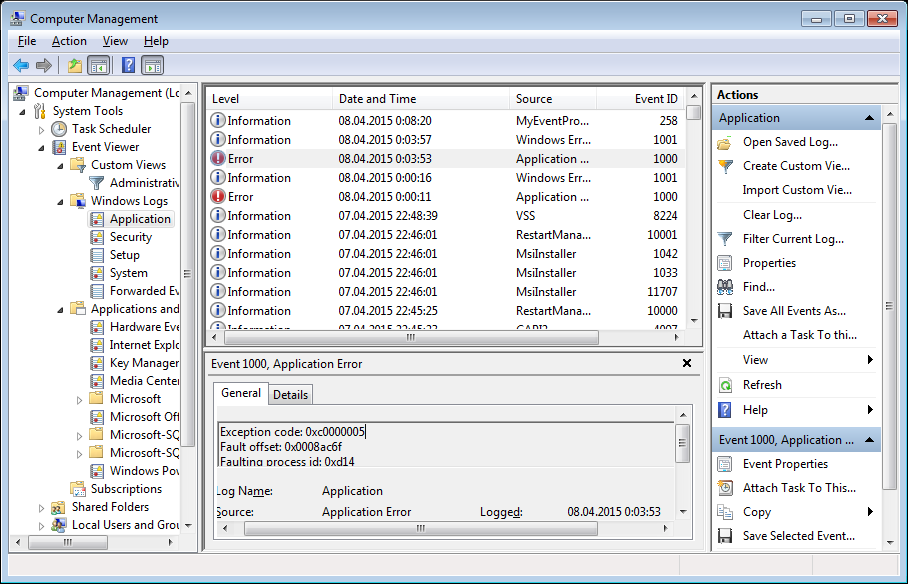
\includegraphics[scale=0.75]{res/managment}
\caption{Просмотру событий системного журнала Windows.}
\end{figure}

В окне просмотра событий отслеживаются сведения в нескольких разных журналах. К журналам Windows относятся следующие:
\begin{itemize}
\item События приложений (программ). В зависимости от важности события делятся на три категории: ошибка, предупреждение или уведомление. Ошибка указывает на серьезную проблему, например потерю данных. Предупреждение указывает на событие, которое в момент записи в журнал не было существенным, но может привести к возникновению проблем в будущем. Информационное событие сообщает об успешной работе приложения, драйвера или службы.
\item События, связанные с безопасностью. Такие события называются аудитами и делятся на успешные или закончившиеся с ошибкой. Они указывают, например, удалось ли пользователю войти в ОС Windows.
\item События установки. Для компьютеров, которые выступают в роли контроллеров домена, здесь отображаются дополнительные журналы.
\item Системные события. Системные события регистрируются Windows и системными службами Windows и подразделяются на ошибки, предупреждения и уведомления.
\item Пересылаемые события. Эти события пересылаются в данный журнал другими компьютерами.
\end{itemize}

Работа с системным журналом Windows значительно сложнее, чем работа с обычным текстовым файлом т.к. требует компиляции ресурс-файлов.

Для создания ресурс-файла нужно в меню проекта вызвать добавление нового файла, указать его тип (текстовый файл) и имя (в моем случае это messages.mc). Рисунок 2 показывает процесс создания этого файла.

Содержимое файла (листинг 1) описывает коды для событий журнала. По представленным комментариям должно быть понятно что происходит: в начале описан язык сообщений (русский) потом две категории сообщений (OVERFLOW\_CATEGORY для событий переполнения при операции над числами с плавающей точкой; OVERFLOW\_CATEGORY для событий деления на ноль) и два определителя сообщений (одно о готовности вызвать исключение, другое о пойманном исключении). Более подробно синтаксис этого файла можно изучить в MSDN \url{https://msdn.microsoft.com/dd996906.aspx}.

\lstinputlisting[language={},caption={Скрипт генерации ресурсов (src/ExceptionsProcessing/WinAPI/messages.mc)}]{../../src/ExceptionsProcessing/WinAPI/messages.mc}

Имея этот скрипт, можно перейти в папку, где он находится, и выполнить команду 

\begin{verbatim}
mc -U messages.mc
\end{verbatim}

\begin{figure}[h!]
\centering
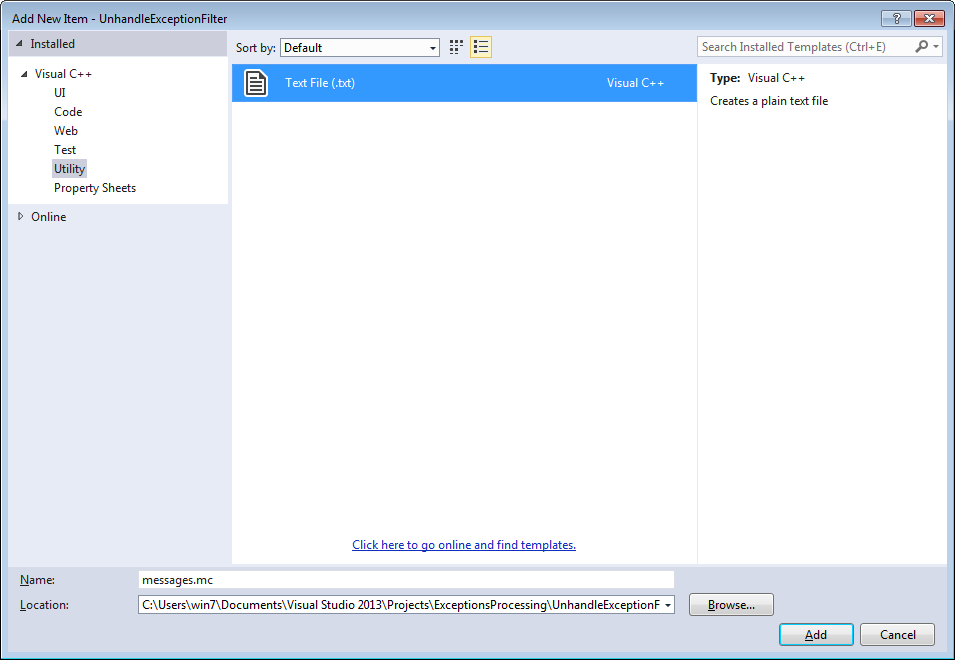
\includegraphics[scale=0.65]{res/message_property0}
\caption{Создание скрипта для генерации ресурсов в проекте.}
\end{figure}

Но можно настроить среду разработки так, чтобы файл компилировался автоматически во время сборки проекта. Для этого нужно вызвать свойства файла messages.mc и в поле "Типа элемента" выбрать "Настраиваемый инструмент построения" (на рисунке 3 этот выбор подсвечен жирным текстом).

\begin{figure}[h!]
\centering
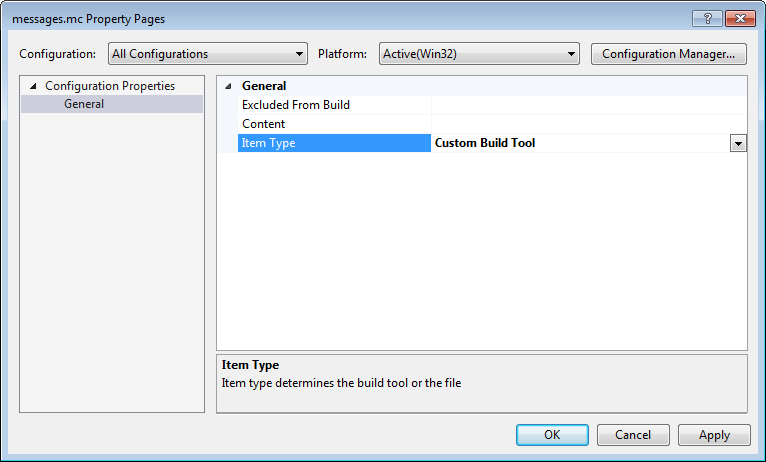
\includegraphics[scale=0.8]{res/message_property1}
\caption{Выбор типа элемента для файла messages.mc}
\end{figure}

После того, как будет нажата кнопка "применить", в левой панели появилась группа "Настраиваемый инструмент построения", где нужно выбрать следующие параметры (смотри рисунок 4):
\begin{verbatim}
Командная строка: mc "%(FullPath)"
Описание: Compiling Messages...
Выводы: %(Filename).rc;%(Filename).h;MSG00419.bin
\end{verbatim}

\begin{figure}[h!]
\centering
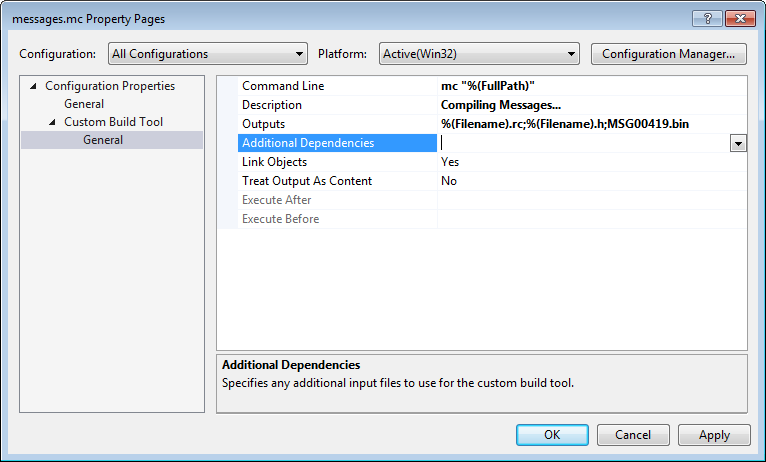
\includegraphics[scale=0.8]{res/message_property2}
\caption{Настройки исполнения скрипта генерации ресурсов}
\end{figure}

Теперь, при сборке проекта, ресурсы будут сгенерированы автоматически:
\begin{itemize}
\item message.h -- заголовочный файл ресурсов (см. листинг 2), его необходимо добавить в проект.
\item message.rc -- файл с описанием ресурсов (моя бесплатная версия Microsoft Visual Studio Express не позволяет редактировать этот файл прямо из среды разработки), необходимо добавить в проект;
\item message.bin -- бинарный файл файл ресурсов.
\end{itemize}

После того, как заголовочный файл (см. листинг 2) будет добавлен в проект, можно будет пользоваться определёнными в нём константами.

\lstinputlisting[language=C++, caption={Заголовочный файл для работы с ресурсами (src/ExceptionsProcessing/WinAPI/messages.h)}]
{../../src/ExceptionsProcessing/WinAPI/messages.h}

После этого с системным журналом уже можно работать, но каждое событие будет начинаться с записи:

\textit{The description for Event ID 258 from source MyEventProvider cannot be found. Either the component that raises this event is not installed on your local computer or the installation is corrupted. You can install or repair the component on the local computer.} (Не удается найти описание для идентификатора события 258 из источника MyEventProvider. Вызывающий данное событие компонент не установлен на этом локальном компьютере или поврежден. Установите или восстановите компонент на локальном компьютере.)

Для исправления этой ситуации нужно сгенерировать библиотеку с ресурсами и зарегистрировать её в системе (см. рис. 5). Это делается при помощи командной строки Visual Studio (Developer Command Prompt for VS2013; не путать с интерпретатором CMD!), в котором делается переход в папку, содержащую messages.res (это может быть папка debug) и выполняется команду
\begin{verbatim}
link /DLL /NOENTRY messages.res
\end{verbatim}

После выполнения этой команды будет создан файл messages.dll.

\begin{figure}[h!]
\centering
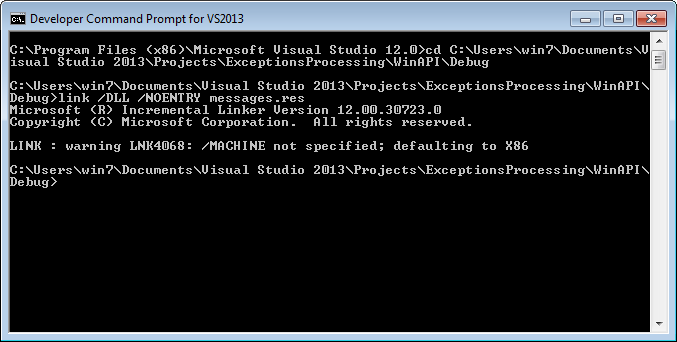
\includegraphics[scale=0.9]{res/res}
\caption{Генерация библиотеки ресурсов}
\end{figure}

При внедрении программы необходимо будет зарегистрировать resources.dll в реестре. Для этого потребуется создать ключ MyEventProvider в ветке реестра HKEY\_LOCAL\_MACHINE$\backslash$\\
SYSTEM$\backslash$CurrentControlSet$\backslash$services$\backslash$eventlog$\backslash$Application и выставить параметры, перечисленные в таблице 1.

\begin{table}[htb]
\begin{tabular}{|c|c|c|c|}
\hline 
Название & Тип & Значение & Примечание \\ 
\hline 
CategoryCount & REG{\_}DWORD & 0x00000002 & количество категорий сообщений \\ 
\hline 
CategoryMessageFile & REG{\_}SZ & path$\backslash$resources.dll & путь до DLL \\ 
\hline 
EventMessageFile & REG{\_}SZ & path$\backslash$resources.dll & путь до DLL \\ 
\hline 
ParameterMessageFile & REG{\_}SZ & path$\backslash$resources.dll & путь до DLL \\ 
\hline 
TypesSupported & REG{\_}DWORD & 0x00000002 & количество типов сообщений \\ 
\hline 
\end{tabular} 
\caption{Значения для заполнения реестра}
\end{table}

Файл с библиотекой стоит перенести в более подходящее место, но общий вид системного реестра должен выглядеть как рисунок 6.

\begin{figure}[h!]
\centering
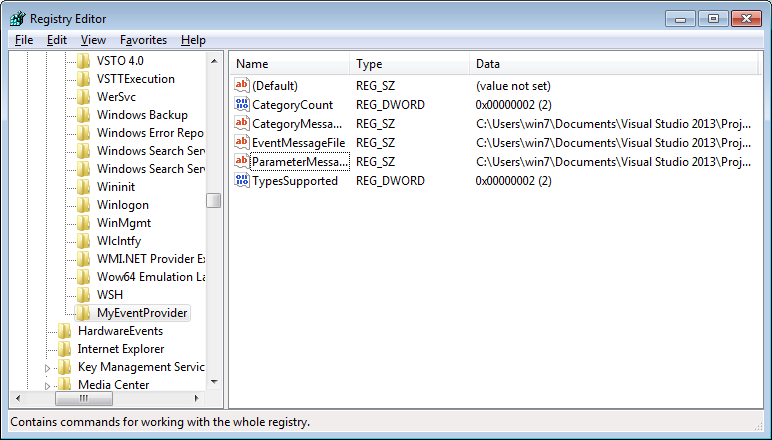
\includegraphics[scale=0.8]{res/reg}
\caption{Редактирование системного реестра}
\end{figure}

После этого события в системном журнале должны отображаются нормально.

Все результаты, представленные в данном отчёте получены с использованием Microsoft Windows 7 Ultimate Service Pack 1 64-bit (build 7601). Для разработки использовалась Microsoft Visual Studio Express 2013 for Windows Desktops (Version 12.0.30723.00 Update 3). В качестве отладчика использовался Microsoft WinDbg (release 6.3.9600.16384), работа с которым будет подробнее рассмотрена на одной из задач.

%------------------------------------------------

\chapter*{Исключения с помощью WinAPI}
\addcontentsline{toc}{chapter}{Исключения с помощью WinAPI}

Задачей этого раздела является генерирование и обработка исключений с помощью функций WinAPI.

В листинге 3 показана работа с исключениями. В зависимости от параметра, передаваемого при запуске, вызывается либо исключение деления на ноль, либо переполнение разрядной сетки при работе с типом float. Особо стоит обратить внимание на две вещи: изначально, все ошибки типа float маскируются, и для получения исключений нужно от этого маскирования избавиться (см. стр. 68-70); кроме того, операции с плавающими точками выполняются асинхронно, и нужно на этапе компиляции отключить расширения векторизации.

В 74-й строке используется квалификатор volatile, это помогает обмануть статический анализатор среды разработки (visual studio), который честно сигнализирует о явной ошибке (делении на ноль) и не позволяет собрать программу.

\lstinputlisting[language=C++, caption={Генерация и обработка исключения с помощью функций WinAPI (src/ExceptionsProcessing/WinAPI/main.cpp)}]
{../../src/ExceptionsProcessing/WinAPI/main.cpp}

Произведём три запуска, первый раз без аргументом (для демонстрации зависимости исключения от передаваемого аргумента), второй раз с аргументом "\-d" (DIVIDE\_BY\_ZERO) и третий раз с аргументом "\-o" (FLT\_OVERFLOW). Как видно на рисунке 7, первый запуск не дал результатов, второй и третий привёл к исключительной ситуации.

\begin{figure}[h!]
\centering
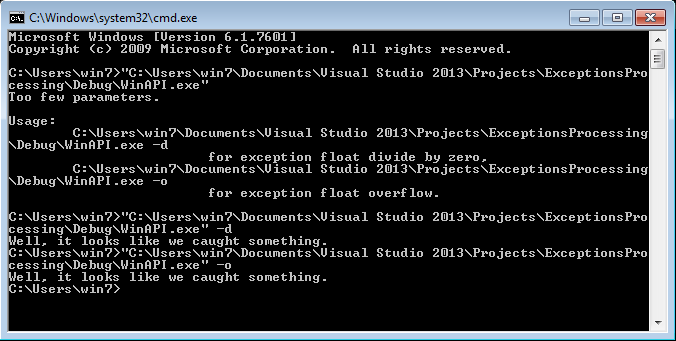
\includegraphics[scale=0.95]{res/001}
\caption{Запуск программы, генерирующей исключения средствами WinAPI.}
\end{figure}

Во время второго и третьего запуска, управление сразу после исключения с 80-й строки (где происходит исключительная ситуация),  передаётся на 97-ю (в которой ожидается исключение), а потом на 104-ю (т.е. обратной передачи управления не происходит), где происходит закрытие используемых дескрипторов и завершение работы. Запись из 81-й и 91-й строк в листинге 4 (лог-файл) отсутствуют, т.к. управление до этих строк не дошло.

В рамках данной задачи мы не разбираем, какое именно исключение произошло, поэтому в системный журнал все пойманные события помечаются как события из группы переполнения.

\lstinputlisting[language={},caption={Генерация и обработка исключения с помощью функций WinAPI}]{res/WinAPI.log}

Из примечательного в этом коде ещё строка 173. В ней показан вызов команды ReportEvent, которая непосредственно передаёт строку в системный журнал. Синтаксис команды следующий:

\begin{verbatim}
BOOL ReportEvent(
  _In_  HANDLE hEventLog,
  _In_  WORD wType,
  _In_  WORD wCategory,
  _In_  DWORD dwEventID,
  _In_  PSID lpUserSid,
  _In_  WORD wNumStrings,
  _In_  DWORD dwDataSize,
  _In_  LPCTSTR *lpStrings,
  _In_  LPVOID lpRawData
);
\end{verbatim}

Значения полей следующие:
\begin{itemize}
\item hEventLog -- описатель логера (инициализирован в строке 22);
\item wType -- тип события (ошибка, предупреждение, успех...);
\item wCategory -- категория события (определяется пользовательским кодом);
\item dwEventID -- определитель события (определяется пользовательским кодом);
\item lpUserSid -- указатель на идентификатор безопасности пользователя (может быть NULL)ж
\item wNumStrings -- количество строк в сообщении события;
\item dwDataSize -- количество байт в прилагаемом бинарном участке;
\item lpStrings -- указатель на массив строк;
\item lpRawData -- указатель на бинарный участок.
\end{itemize}

В случае успеха, функция возвращает не нулевой результат. Увидеть зафиксированное событие можно на рисунке 8. Информация события представляет меньше полезной информации, чем лог-файл, так что далее все события будут сохраняться в папку logs, но в отчёте приводиться не будут.

\begin{figure}[h!]
\centering
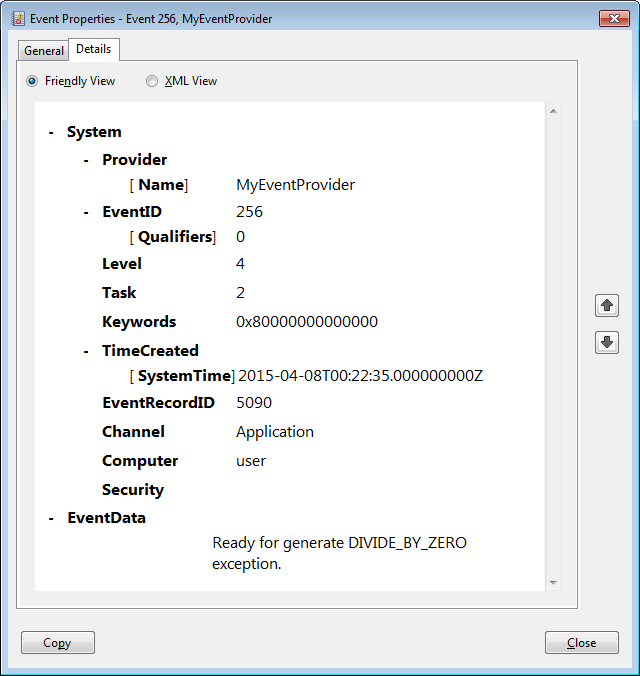
\includegraphics[scale=0.8]{res/event}
\caption{Просмотр события в "дружелюбном" виде (альтернативой которому является XML).}
\end{figure}


Теперь можно перейти к отладке кода при помощи WinDbg.

WinDbg — позволяет отлаживать 32/64 битные приложения пользовательского уровня, драйвера, может быть использован для анализа аварийных дампов памяти, WinDbg поддерживает автоматическую загрузку отладочных символов, имеется встроенный скриптовый язык для автоматизации процесса отладки, а самое главное распространяется корпорацией Microsoft совершенно бесплатно.

В отличии от OllyDbg, WinDbg при первом запуске имеет достаточно неприятный интерфейс и требуется довольно много усилий и времени для подготовки этого инструмента к комфортной работе. На рисунке 9 можно увидеть интерфейс WinDbg и запущенную программу WinAPI.

\begin{figure}[h!]
\centering
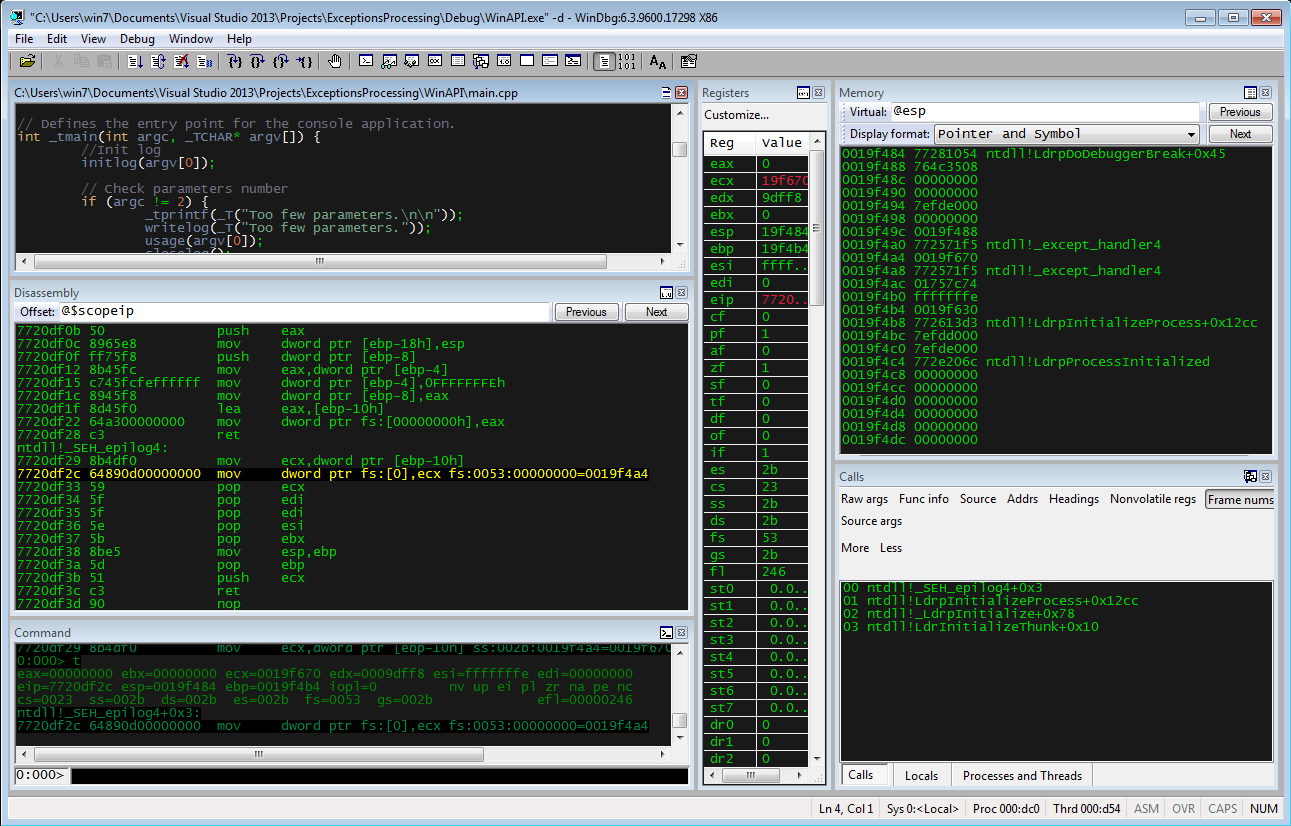
\includegraphics[scale=0.5]{res/002}
\caption{Запуск WinAPI.exe под отладчиком WinDbg.}
\end{figure}

Экран разделён на три участка. В левой части представлены три окна: окно исходного кода (там отображаются даже комментарии на русском языке), под ним окно с ассемблерным кодом (имеется возможность устанавливать точки основа как в кода не С, так и в ассемблерном коде), а под ним диалоговое окно, в котором отображается результат выполнения запросов пользователя. Центральное окно представляет таблицу значений регистров центрального процессора. В правой части снова три окна: два верхних показывают состояние памяти (но можно выбрать представление, допустим в одном случае память выглядит как набор байтов, а в другом как юникод - это удобно для быстрого переключения между различными сегментами), а под ними окно стека.

Контроль исполнения:
\begin{itemize}
\item g -- продолжить выполнение.
\item p -- шаг через функцию.
\item t -- шаг внутрь функции.
\item pa addr -- шаг в адрес.
\item pc -- шаг в следующий вызов.
\item pt -- шаг к следующему возврату.
\item pct -- шаг к следующему вызову или возврату.
\end{itemize}

Точки останова:
\begin{itemize}
\item bp -- установка точки останова, например bp nt!NtCreateFile.
\item bl -- список точек останова.
\item bd -- <число> убрать точку останову под номером.
\item bc -- <число> очистить точку останова под номером.
\item ba -- точка останова на доступ.
\item be -- точка останова на исполнение.
\item bw -- точка останова на запись.
\item sxe ld:kernel32 -- точка останова на загрузке DLL модуля.
\end{itemize}

Работа с дампом (в данной работе не требуется, но для полноты картины):
\begin{itemize}
\item d <адрес> -- дамп памяти по адресу (b-byte;w-word;d-dword).
\item dd <регистр> -- дамп содержимого регистра.
\item ddp <адрес> -- дамп содержимого по адресу.
\item u <адрес> -- дизассемблировать по адресу.
\end{itemize}

Передачу управления можно видеть и по средствам отладчика. В правом нижнем углу показан стек. В данном случае глубина стека не достаточно большая для наглядного изучения поиска обработчика, но вызов обработчика на нём виден.

Благородя тому, что исключение было обработано, оно не дошло до уровня операционной системы, и не было отражено в системном журнале как ошибка.

%------------------------------------------------

\chapter*{Использование GetExceptionCode}
\addcontentsline{toc}{chapter}{Использование GetExceptionCode}

Функция GetExceptionCode позволяет получить код исключения, которое было сгенерировано в процессе работы программы (смотри листинг 5). В первом случае (строка 86) она участвует в сравнении с макро-константной EXCEPTION\_FLT\_DIVIDE\_BY\_ZERO для определения подходящего обработчика для исключительного события. Во-втором случае (строка 109) она используется уже внутри обработчика, позволяя определить, что исключение вызвано переполнением при операции с типом float.

\lstinputlisting[language=C++, caption={Получение кода исключения с помощью функции GetExceptionCode (src/ExceptionsProcessing/GetExceptionCode/main.cpp)}]
{../../src/ExceptionsProcessing/GetExceptionCode/main.cpp}

Таким образом, рассмотрены два способа фильтрации исключений - на уровне входа в блок \_\_except, либо уже непосредственно в обработчике (тогда в \_\_except ставится макро-константа EXCEPTION\_EXECUTE\_HANDLER, позволяющая принимать любые исключения). Далее будет рассмотрен более логичный способ фильтрации исключений специальной функцией.

Запуск под отладчиком показывает картину практически аналогичную предыдущему случаю, но есть разница в логе работы программы (листинг 6). На этот раз мы знаем какое исключение произошло и это фиксируем в логе.

\lstinputlisting[language={},caption={Генерация и обработка исключения с помощью функций WinAPI}]{res/GetExceptionCode.log}

%------------------------------------------------

\chapter*{Пользовательская функция-фильтр}
\addcontentsline{toc}{chapter}{Пользовательская функция-фильтр}

В листинге 7 представлена функция-фильтр, которая возвращает \\ EXCEPTION\_CONTINUE\_SEARCH только если исключение вызвано \\ EXCEPTION\_FLT\_DIVIDE\_BY\_ZERO или EXCEPTION\_FLT\_OVERFLOW.

\lstinputlisting[language=C++, caption={Использование собственной функции фильтра (src/ExceptionsProcessing/FilterFunction/main.cpp)}]
{../../src/ExceptionsProcessing/FilterFunction/main.cpp}

При изучении работы программы под отладчиком, выяснилось что при возникновении исключения, управление не передаётся в то место, где определена функция-фильтр. Вероятно компилятор оптимизирует код и подставляет её целиком на место вызова. На рисунке 10 видна передача управления на обработку исключения после работы функции-фильтра.

\begin{figure}[h!]
\centering
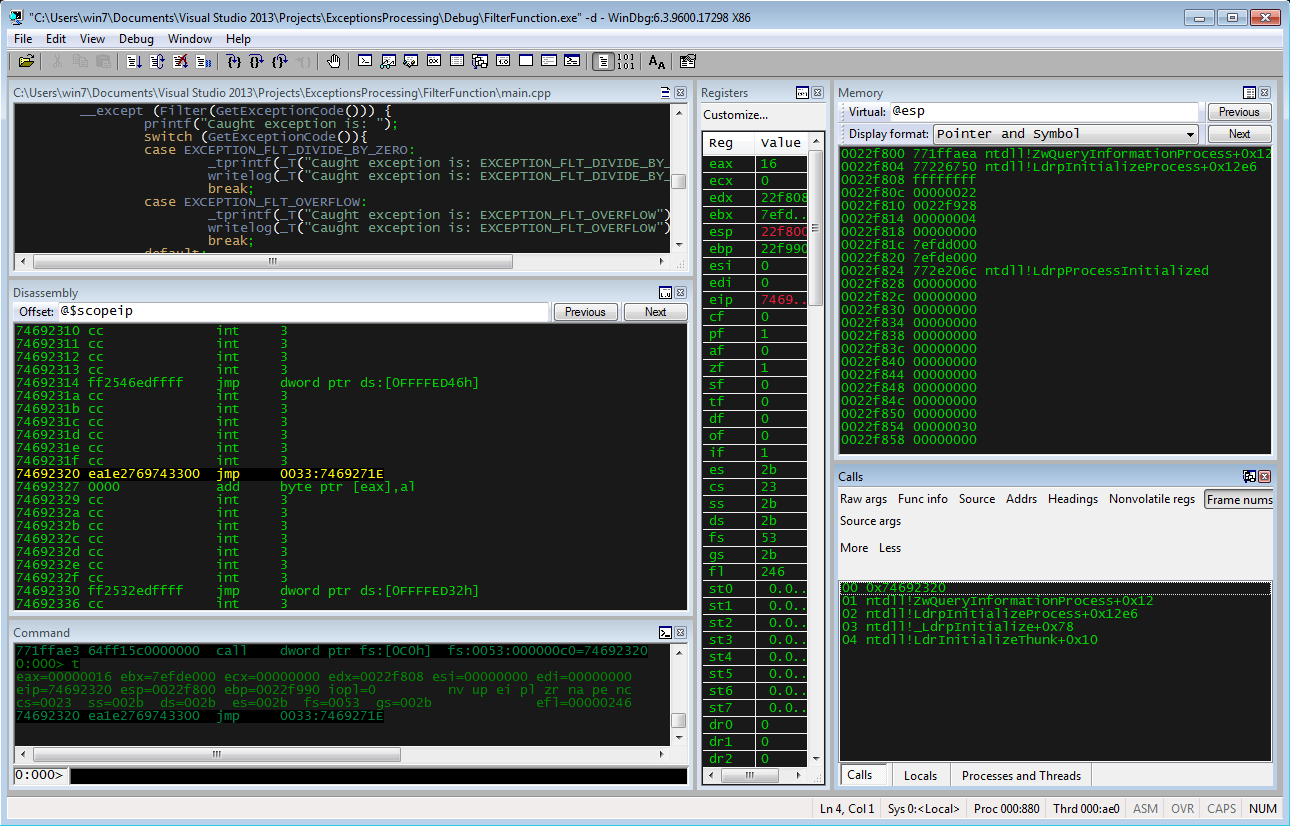
\includegraphics[scale=0.5]{res/003}
\caption{Передача управления обработчику, после отработки функции-фильтра}
\end{figure}

В обработчике фактически происходит только вызов функций логирования (листинг 8). Как и раньше, строки 82 и 92 оказываются пропущенными, т.к. после возбуждения исключения управление переходит обработчику, нарушая линейный порядок.

\lstinputlisting[language={},caption={Генерация и обработка исключения с помощью функций WinAPI}]{res/FilterFunction.log}

%------------------------------------------------

\chapter*{Использование RaiseException}
\addcontentsline{toc}{chapter}{Использование RaiseException}

Исключение можно возбудить не только в результате каких-то арифметических или логических операций, но и искусственным образом, вызвав функцию RaiseException. Она обладает 4-я параметрами, но наиболее важным является первый, который определяет тип возбуждаемого исключения. Работа этой функции показана в листинге 9.

\lstinputlisting[language=C++, caption={Программная генерация исключения при помощи функции RaiseException (src/ExceptionsProcessing/RaiseException/main.cpp)}]
{../../src/ExceptionsProcessing/RaiseException/main.cpp}

Информацию об исключении можно получить из функции GetExceptionInformation, которая, в действительности, никакой информацией не владеет но возвращает указатель на структуру EXCEPTION\_POINTERS. В свою очередь, эта структура содержит два указателя на ExceptionRecord и на ContextRecord, в которых уже находится информация об исключении.

Важной особенностью функции GetExceptionlnformation является то, что ее можно вызывать только в функции-фильтре исключений, т.к. структуры CONTEXT, EXCEPTION\_RECORD и EXCEPTION\_POINTERS существуют лишь во время обработки фильтра исключения. В момент, когда управление переходит к обработчику исключений, эти данные в стеке разрушаются. На рисунке 11 показан момент получения информации о возникшем исключении. Обработчик исключения находится выше по стеку, и когда ему будет возвращено управление от функции фильтра стек уже будет зачищен.

\begin{figure}[h!]
\centering
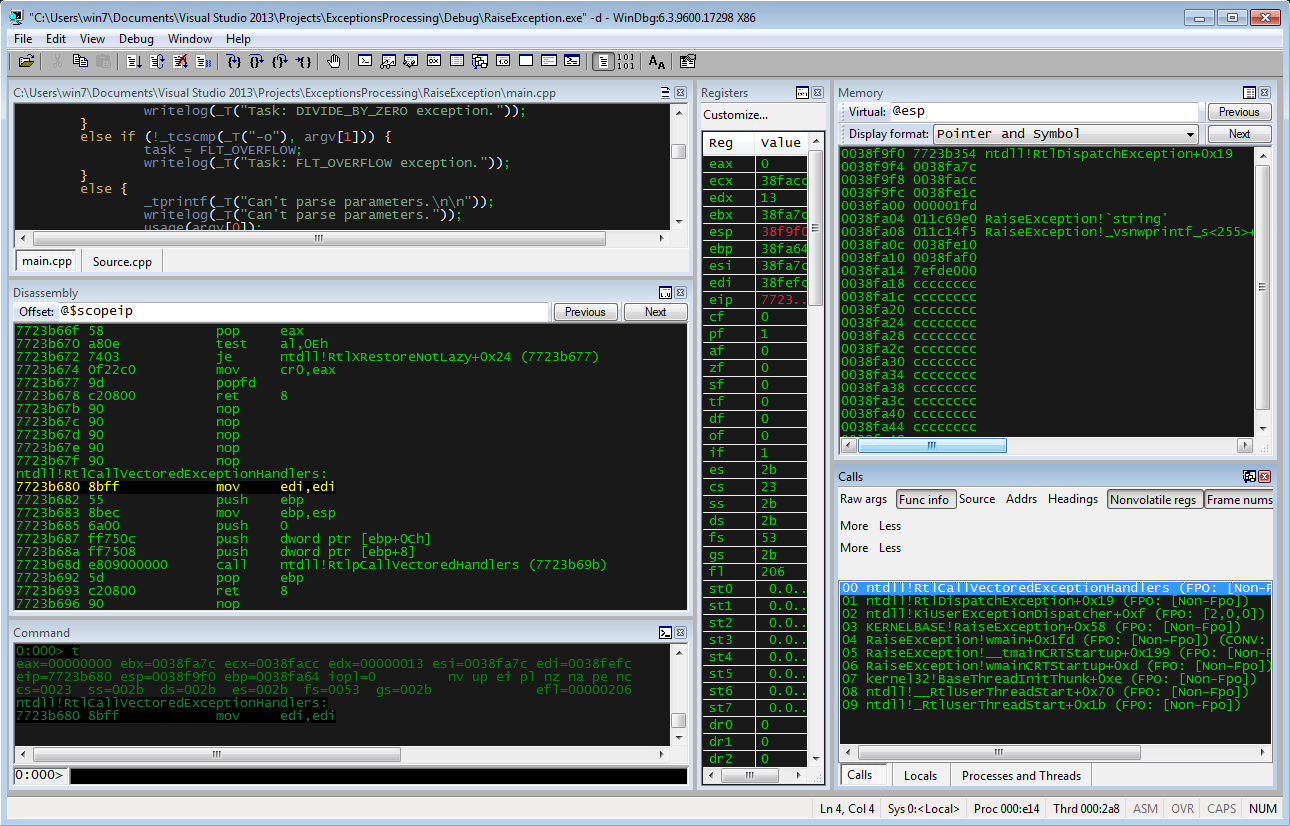
\includegraphics[scale=0.5]{res/005}
\caption{Информация об исключении доступна в процессе работы функции-фильтра}
\end{figure}

\newpage

\begin{figure}[h!]
\centering
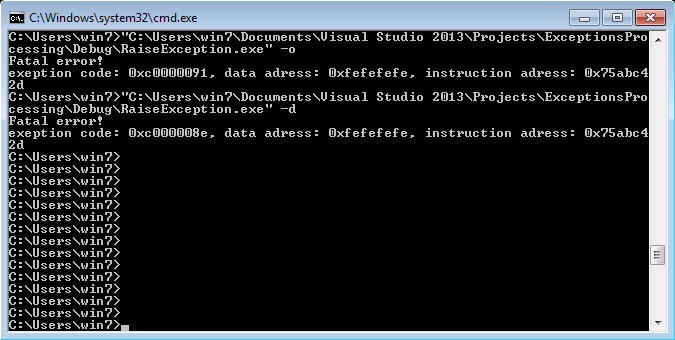
\includegraphics[scale=0.95]{res/004}
\caption{Передача управления обработчику, после отработки функции-фильтра}
\end{figure}

На рисунке 12 показан вызов программы, генерирующей исключения программным образом, а в листинге 10 представлен лог её работы.

\lstinputlisting[language={},caption={Программная генерация исключения и получение информации о нём}]{res/RaiseException.log}

%------------------------------------------------

\chapter*{Необрабатываемые исключения}
\addcontentsline{toc}{chapter}{Необрабатываемые исключения}

Если ни один из установленных программистом обработчиков не подошла для обработки исключения (либо программист вообще не установил ни один обработчик), то вызывается функция UnhandledExceptionFilter, которая выполняет проверку, запущен ли процесс под отладчиком, и информирует процесс, если отладчик доступен. Далее, функция вызывает фильтр умалчиваемого обработчика (который устанавливается функцией SetUnhandledExceptionFilter и который возвращает EXCEPTION\_EXECUTE\_HANDLER). Затем, в зависимости от настроек операционной системы, вызывается либо отладчик, либо функция NtRaiseHardError, которая отображает сообщение об ошибке. 

Листинг 11 показывает работу с UnhandledExceptionFilter. Возвращаемое значение определяется в строках 119 и 120.

\lstinputlisting[language=C++, caption={Необработанные исключения\\ (src/ExceptionsProcessing/UnhandleExceptionFilter/main.cpp)}]
{../../src/ExceptionsProcessing/UnhandleExceptionFilter/main.cpp}

Для начала запустим программу так, чтобы фильтр возвращал EXCEPTION\_EXECUTE\_HANDLER. Это считается нормальной ситуацией, и на рисунке 13 видно как происходит передача управления.

\begin{figure}[h!]
\centering
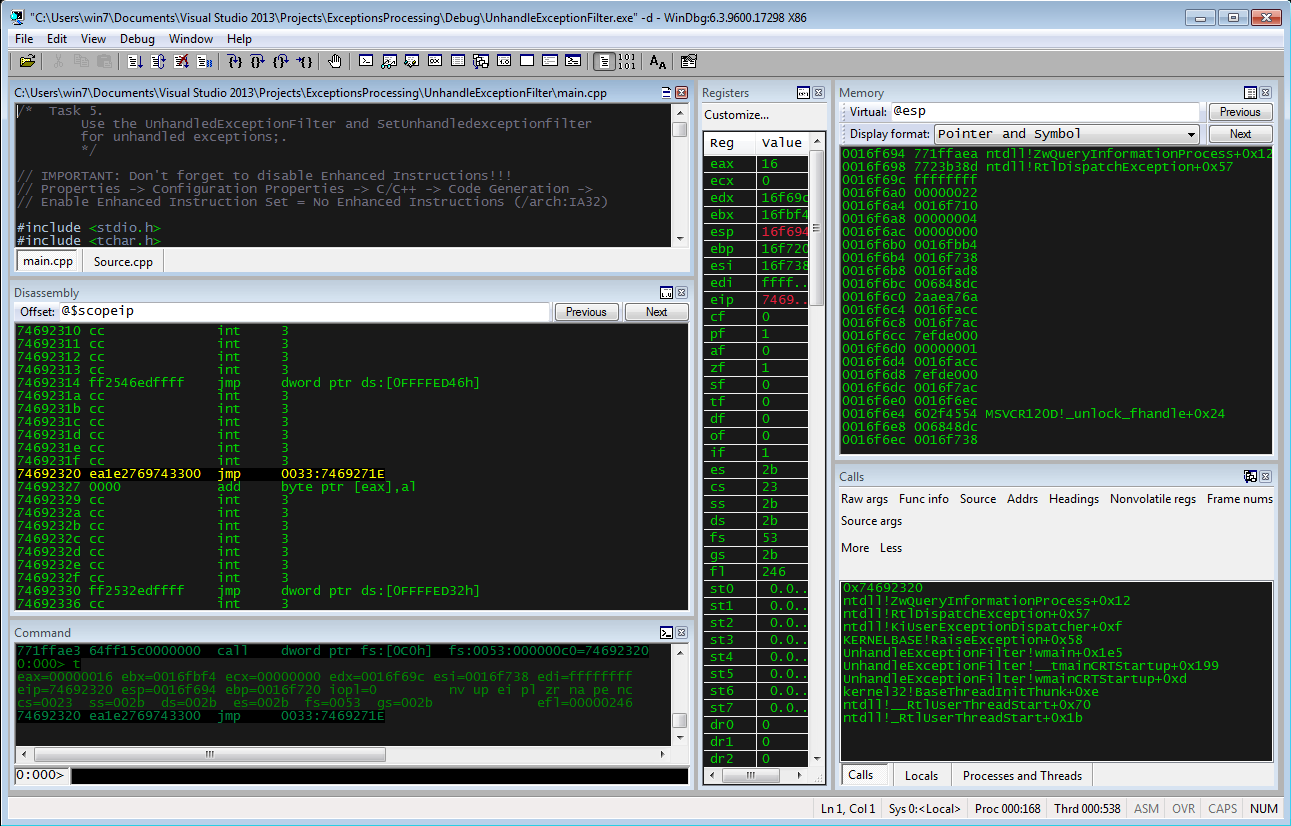
\includegraphics[scale=0.5]{res/006}
\caption{Нормальная обработка исключения через фильтр}
\end{figure}

Запустим программу ещё раз,  фильтр вернёт EXCEPTION\_CONTINUE\_SEARCH. Это событие будет передано операционной системе, и будет зафиксировано в системном журнале (рисунок 14). Что примечательно, обработчик успел выполнить свою задачу, информация об ошибке выведена на экран (рисунок 15) и сохранена в лог (листинг 12), системная ошибка возникла уже после.
\newpage

\begin{figure}[h!]
\centering
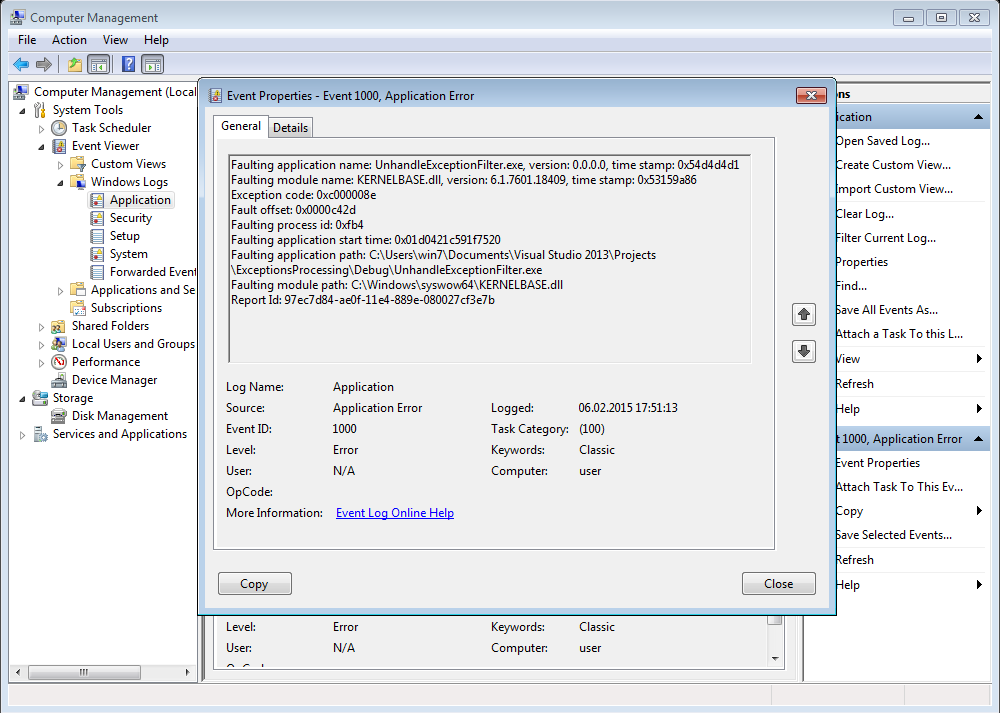
\includegraphics[scale=0.63]{res/007}
\caption{Исключение зафиксировано в системном журнале}
\end{figure}

\begin{figure}[h!]
\centering
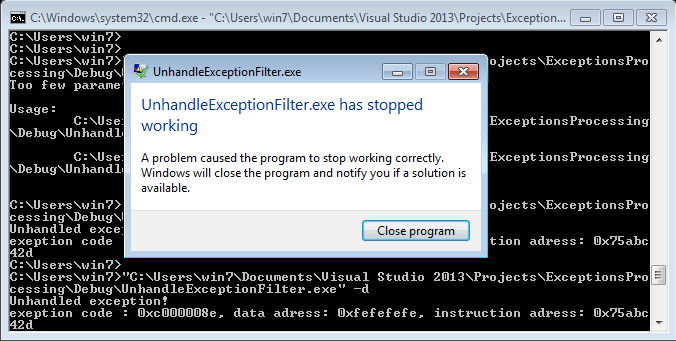
\includegraphics[scale=0.8]{res/008}
\caption{Обработчик успел выполниться до системной ошибки}
\end{figure}

В логе программы можно прочитать информацию о произошедшей исключительной ситуации. Вместе с тем, можно видеть, что программа не была завершена корректно, а дескриптор файла-лога не был закрыт.

\lstinputlisting[language={},caption={Обработчик успел сохранить данные об исключении}]{res/UnhandleExceptionFilter.log}

Из рассмотренного примера становится видно, что возврат EXCEPTION\_EXECUTE\_HANDLER является более предпочитаемым результатом, т.к. исключение нужно обрабатывать там, где оно возникло.

%------------------------------------------------

\chapter*{Вложенные исключения}
\addcontentsline{toc}{chapter}{Вложенные исключения}

Листинг 13 показывает, как происходит передача исключения, в поисках подходящего обработчика. Самым ближайшим (по стеку) обработчиком для исключения, вызванного делением на 0, является обработчик из 48-й строки. Но там стоит ограничение, позволяющее обрабатывать только исключения, вызванные переполнением. В результате обработка этого исключения передаётся в 58-ю строку, хотя этот обработчик дальше по стеку.

\lstinputlisting[language=C++, caption={Вложенные исключения (src/ExceptionsProcessing/NestedException/main.cpp)}]
{../../src/ExceptionsProcessing/NestedException/main.cpp}

Запуск отладчика подтвердил ожидаемый результат - поиск подходящего обработчика для исключения происходит снизу вверх. В начале проверяется ближайший обработчик (на рисунке 16 отрабатывает фильтр ближайшего обработчика исключения). Эта проверка вернёт EXCEPTION\_CONTINUE\_SEARCH для продолжения поиска более подходящего обработчика и передачи управления дальше по стеку.
\newpage

\begin{figure}[h!]
\centering
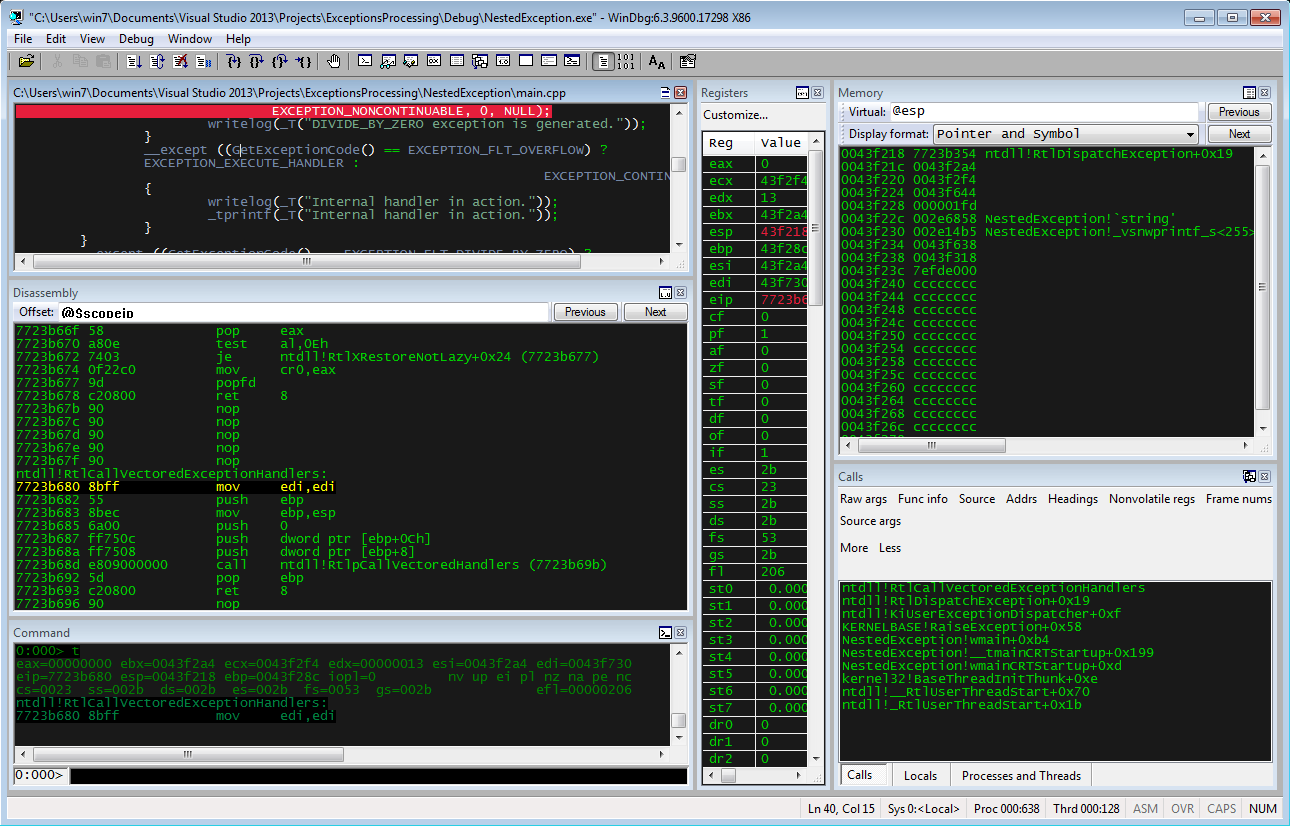
\includegraphics[scale=0.50]{res/009}
\caption{Проверка условий обработчика исключения}
\end{figure}

При этом создаётся опасность утечки ресурсов, поэтому желательно обрабатывать исключительные ситуации в месте их возникновения. Протокол работы программы показан в листинге 14.

\lstinputlisting[language={},caption={Обработчик успел сохранить данные об исключении}]{res/NestedException.log}
%------------------------------------------------

\chapter*{Выход при помощи goto}
\addcontentsline{toc}{chapter}{Выход при помощи goto}

Использование goto считается дурной практикой по целому ряду причин. В листинге 15, благодаря goto управление со строки 40 передаётся сразу на строку 55. Таким образом осуществляется выход из блока \_\_try без возбуждения и обработки исключения.

\lstinputlisting[language=C++, caption={Выход из блока охраняемого кода при помощи goto (src/ExceptionsProcessing/Goto/main.cpp)}]
{../../src/ExceptionsProcessing/Goto/main.cpp}

\begin{figure}[h!]
\centering
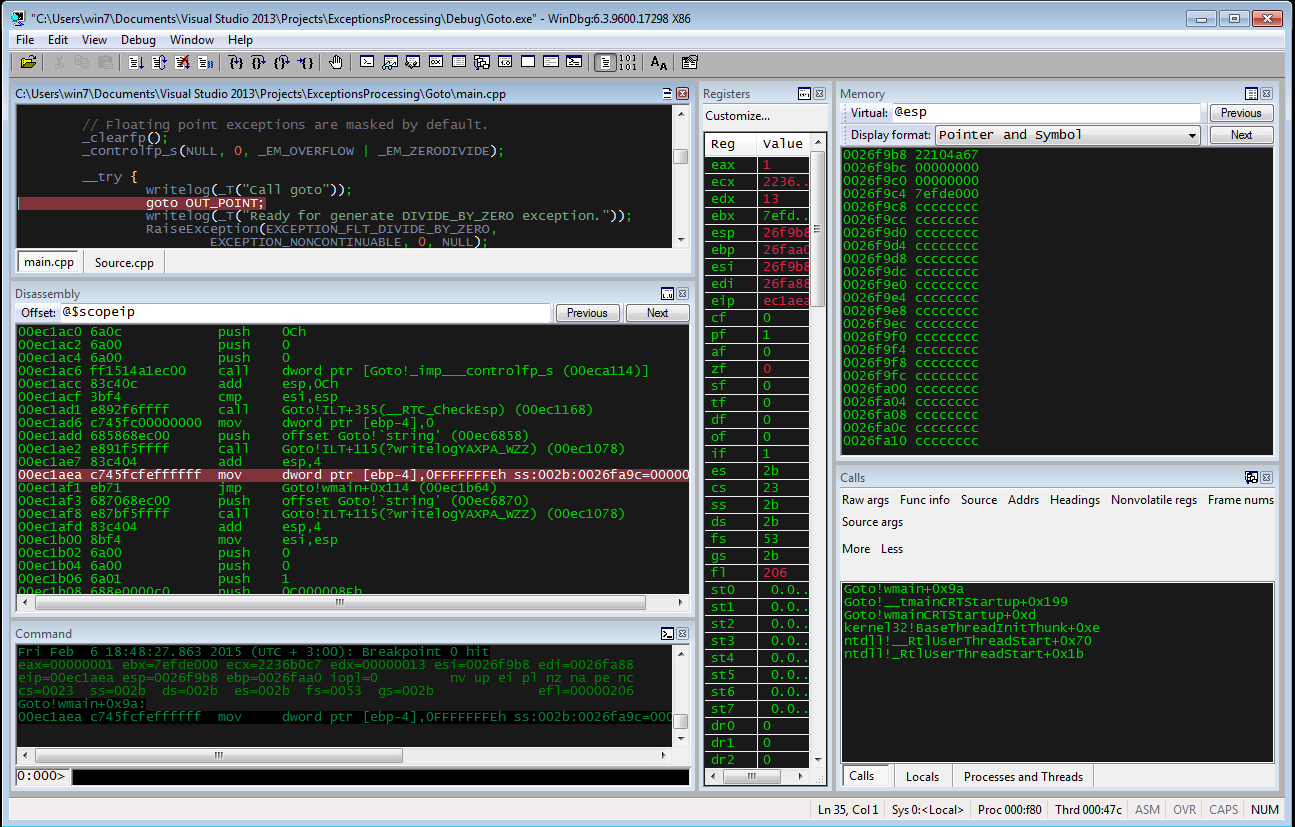
\includegraphics[scale=0.50]{res/010}
\caption{Переход по goto}
\end{figure}

На рисунке 17 видно, что как только достигнута строка с оператором goto, осуществляется безусловный переход к метке. Протокол работы программы (листинг 16) подтверждает, что до возбуждения исключения управление не дошло: после записи  логе из 40-й строки идёт запись из 55-й, таким образом строки 44-46 пропущены.
\newpage

\lstinputlisting[language={},caption={Переход по оператору goto}]{res/Goto.log}

Использование goto может привести к утечкам памяти в процессе раскрутки стека, в то же время он позволяет сделать переход сразу через несколько участков кода. Таким образом, сфера применения goto достаточно узкая, и требует достаточно чёткого понимания.
%------------------------------------------------

\chapter*{Выход при помощи \_\_leave}
\addcontentsline{toc}{chapter}{Выход при помощи \_\_leave}

Листинг 17 похож на листинг 15, но за пределы охраняемого фрейма кода помогает выйти на этот раз \_\_leave. Оператор \_\_leave более эффективен, поскольку не вызывает разрушение стека.

\lstinputlisting[language=C++, caption={Выход из блока охраняемого кода при помощи \_\_leave (src/ExceptionsProcessing/Leave/main.cpp)}]
{../../src/ExceptionsProcessing/Leave/main.cpp}

\begin{figure}[h!]
\centering
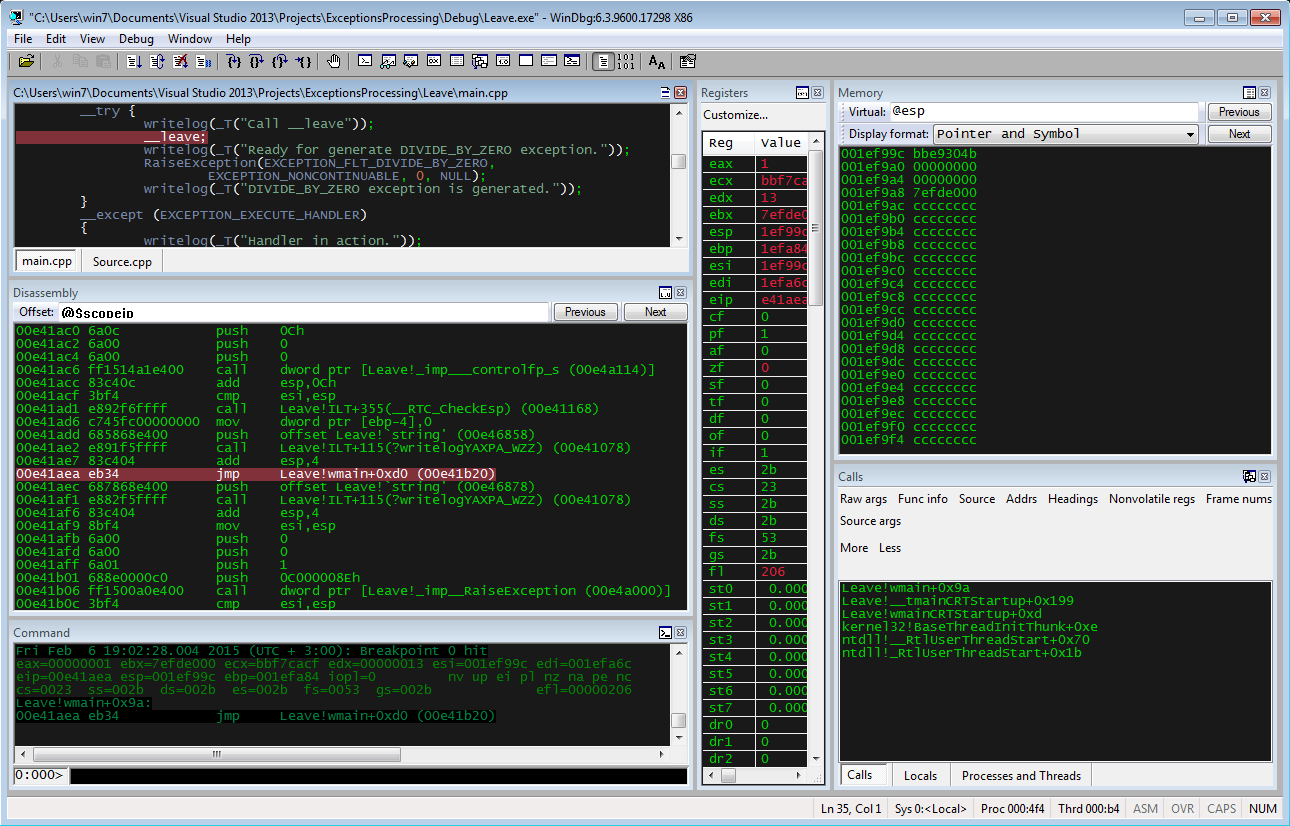
\includegraphics[scale=0.50]{res/011}
\caption{Переход по \_\_leave}
\end{figure}

\lstinputlisting[language={},caption={Переход по оператору \_\_leave}]{res/Leave.log}

Результат использования \_\_leave — переход в конец блока try (грубо говоря, это можно рассматривать это как goto переход на закрывающую фигурную скобку блока try и вход в блок finally естественным образом). По сути, результат прежний (если смотреть на листинг 18), но метод его достижения отличается -- этот способ считается более правильным, т.к. не приводит к раскрутке стека.

После перехода выполняется обработчик завершения. Хотя для получения того же результата можно использовать оператор goto, он (оператор goto) приводит к освобождению стека. Одним из применений этого оператора является трассировка программ.

%------------------------------------------------

\chapter*{Преобразование SEH в C++ исключение}
\addcontentsline{toc}{chapter}{Преобразование SEH в C++ исключение}

Листинг 19 показывает встраивание SEH в механизм исключений C/С++. Для этого необходимо включить соответствующие опции в компиляторе (/EHa).

\lstinputlisting[language=C++, caption={Трансформация исключений (src/ExceptionsProcessing/Translator/main.cpp)}]
{../../src/ExceptionsProcessing/Translator/main.cpp}

На рисунке 19 видна передача управления от генерации исключения в ядре к созданию пользовательского исключения. Листинг 20 показывает, какие участи кода были задействованы и в каком порядке.

\begin{figure}[h!]
\centering
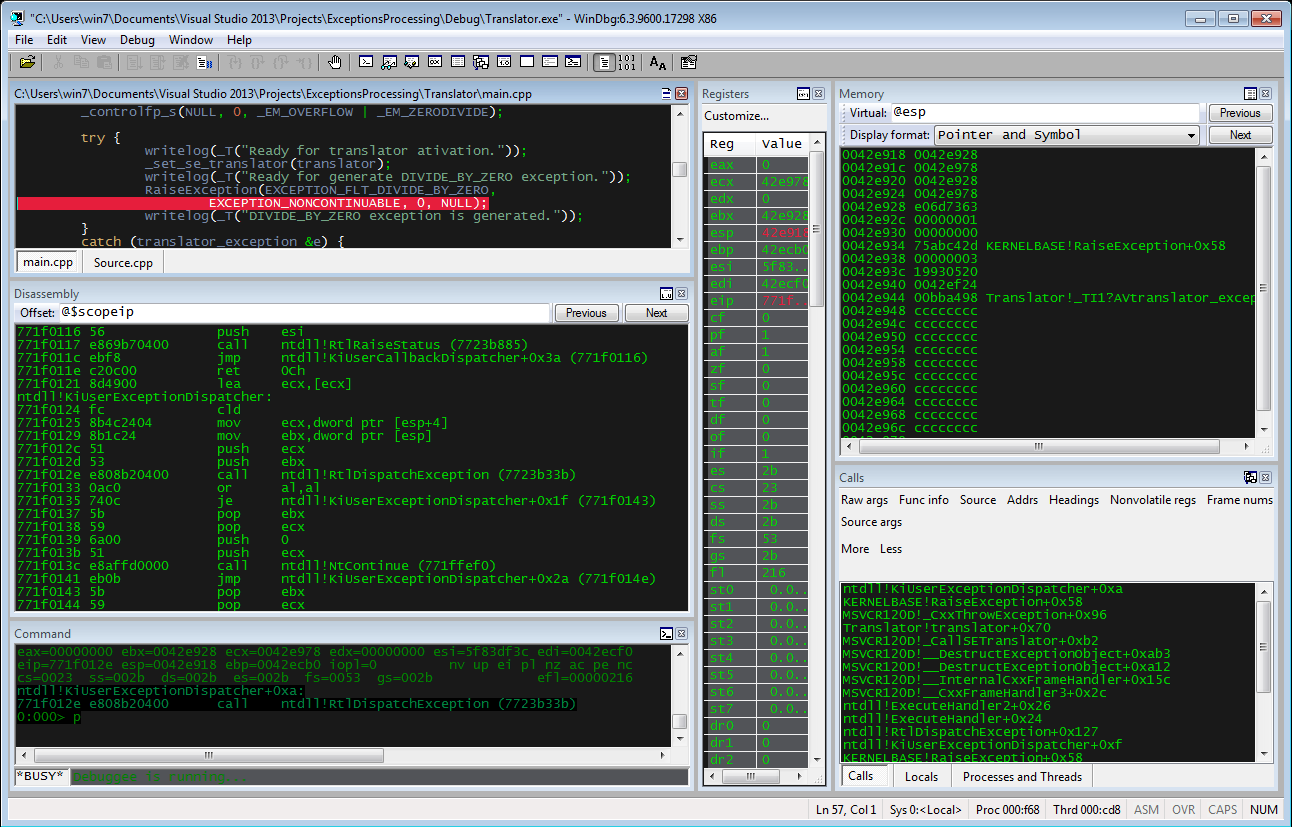
\includegraphics[scale=0.50]{res/012}
\caption{Передача управления коду создания пользовательского исключения}
\end{figure}
\newpage

\lstinputlisting[language={},caption={Результат работы Translator.exe}]{res/Translator.log}

Если проследить за передачей управления по стеку вызовов, то сразу после возбуждения исключения в 63-й строке, управление передаётся транслятору, где генерируется привычное С++-исключения (в данном случае используется собственный класс исключения, определённый в 37-й строке), и только после этого в блок catch, где происходит обработка исключения.

Этот механизм способен обеспечить взаимодействие SEH с другими языками и системами.
%------------------------------------------------

\chapter*{Финальный обработчик finally}
\addcontentsline{toc}{chapter}{Финальный обработчик finally}

В листинге 21 исключение как таковое отсутствует, но есть охраняемый блок кода, и блок \_\_finally, управление в который будет передано в любой ситуации.

\lstinputlisting[language=C++, caption={Исполнение кода в блоке \_\_finally (src/ExceptionsProcessing/Finally/main.cpp)}]
{../../src/ExceptionsProcessing/Finally/main.cpp}

\begin{figure}[h!]
\centering
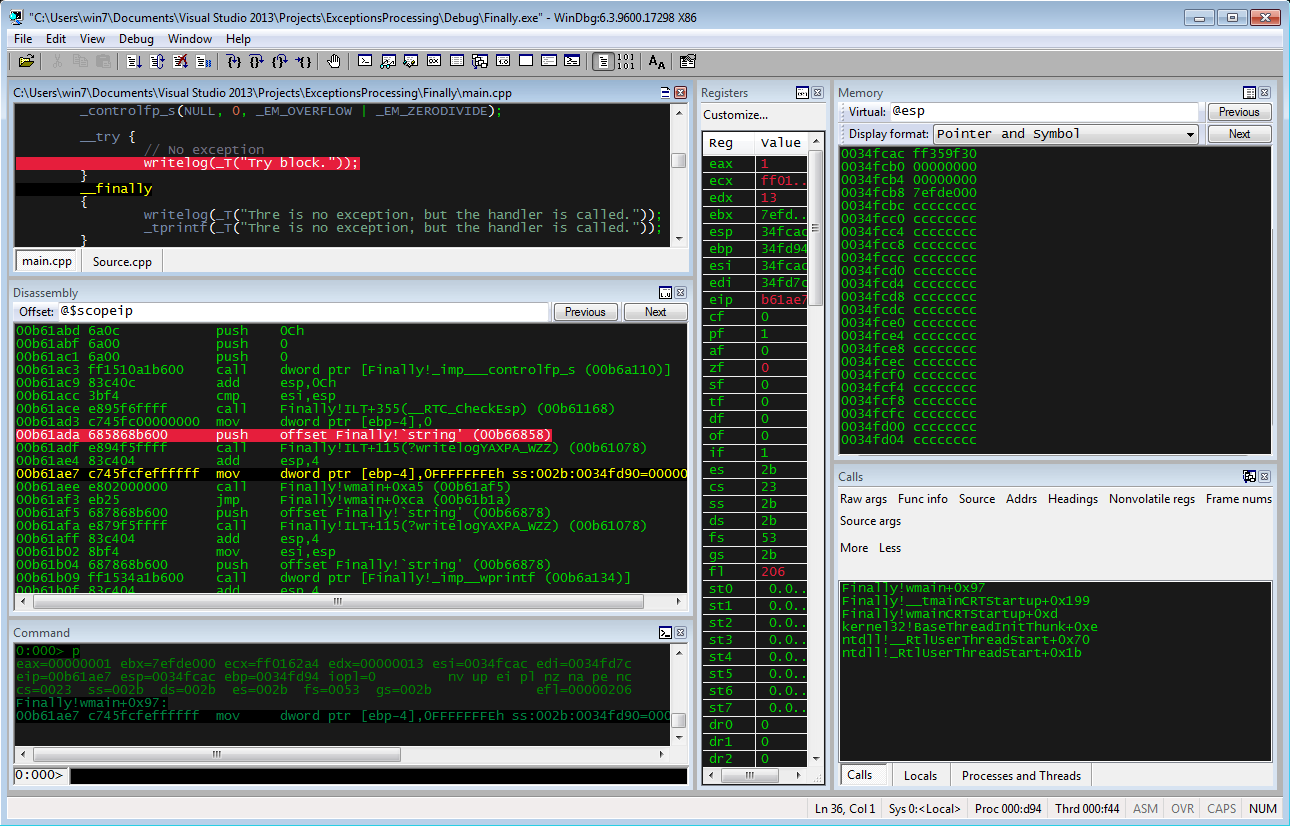
\includegraphics[scale=0.50]{res/013}
\caption{Переход в блок finally}
\end{figure}

\lstinputlisting[language={},caption={Результат работы Finally.exe}]{res/Finally.log}

Вместо передачи управления обратно в программу, управление передаётся в блок \_\_finally (рисунок 20). Более того, управление туда будет передано даже если блок защищаемого кода будет пуст. Листинг 22 показывает порядок исполнения кода.

Похожие механизмы есть в других распространённых языках программирования, они позволяют обеспечить строгие гарантии исключений, и не допустить нахождение объекта в не консистентном состоянии.
\newpage
%------------------------------------------------

\chapter*{Использование функции AbnormalTermination}
\addcontentsline{toc}{chapter}{Использование функции AbnormalTermination}

В листинге 23 сравниваются два механизма из блока \_\_try. Благодаря тому, что управление будет передано блоку \_\_finally в любом случае, оказывается удобно в этом блоке проверять корректность выхода из блока \_\_try (при помощи функции AbnormalTermination), и, в случае необходимости, корректно освобождать захваченные ресурсы.

\lstinputlisting[language=C++, caption={Проверка корректности выхода из блока \_\_try (src/ExceptionsProcessing/AbnormalTermination/main.cpp)}]
{../../src/ExceptionsProcessing/AbnormalTermination/main.cpp}

\begin{figure}[h!]
\centering
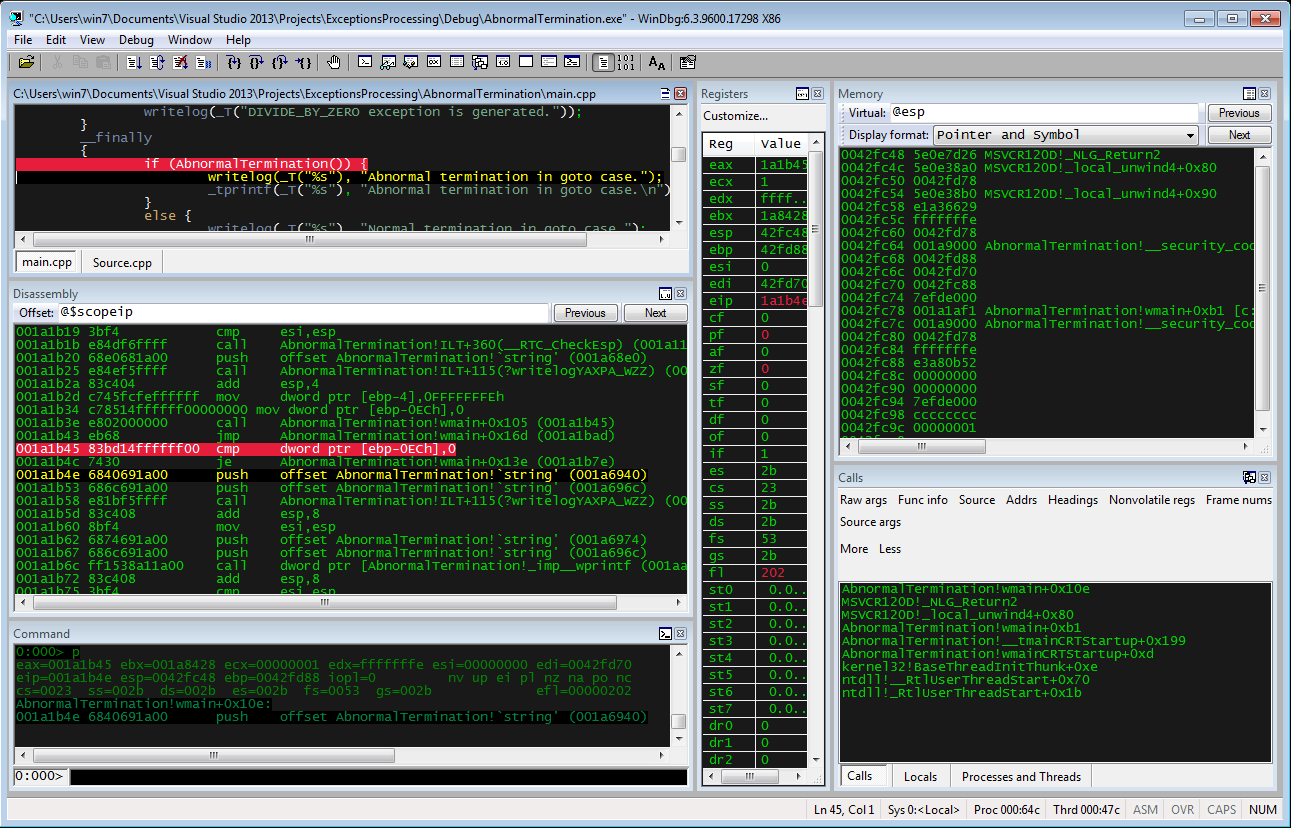
\includegraphics[scale=0.50]{res/014}
\caption{Выход из защищаемого блока по goto}
\end{figure}

\begin{figure}[h!]
\centering
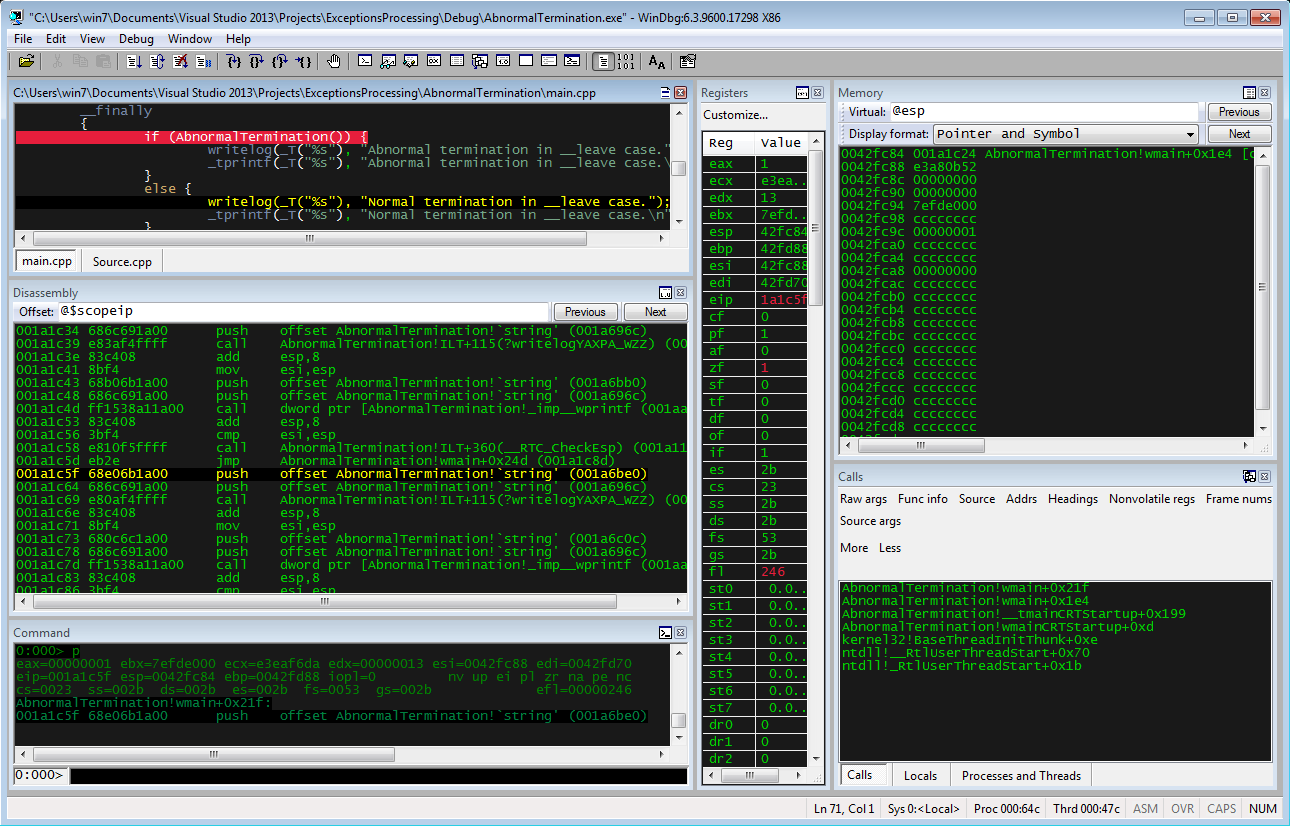
\includegraphics[scale=0.50]{res/015}
\caption{Выход из защищаемого блока по \_\_leave}
\end{figure}


Функция AbnormalTermination() позволяет определить на сколько правильным был выход из защищаемого кода в случае с goto (рисунок 21) и \_\_leave (рисунок 22). Протокол работы программы представлен в листинге 22.
\newpage

В зависимости от этого принимается решение об освобождении захваченных ресурсов, но если по какой-то причине нужно выйти из защищаемого блока (хотя причина такой необходимости не очевидна) лучше использовать \_\_leave, т.к. с goto больше шансов на утечку ресурсов, захваченных (и не освобождённых) в блоке \_\_try.

\lstinputlisting[language={},caption={Результат работы Finally.exe}]{res/AbnormalTermination.log}

%------------------------------------------------

\chapter*{Заключение}
\addcontentsline{toc}{chapter}{Заключение}

\vspace{3em}
При обработке исключений в С++ используются ключевые слова catch и throw, а сам механизм исключений реализован с использованием SEH. Тем не менее, обработка исключений в С++ и SEH — это разные вещи. Их совместное применение требует внимательного обращения, поскольку обработчики исключений, написанные пользователем и сгенерированные C++, могут взаимодействовать между собой и приводить к нежелательным последствиям. Документация Microsoft рекомендует полностью отказаться от использования обработчиков Windows в прикладных программах на С++ и ограничиться применением в них только обработчиков исключений С++.

\vspace{2em}
Кроме того, обработчики исключений или завершения Windows не осуществляют вызов деструкторов, что в ряде случаев необходимо для уничтожения экземпляров объектов С++.

\vspace{2em}
В то же время, наличие таких мощных инструментов как блок \_\_finally, гибкая система фильтрации и извлечение контекста исключения делает их незаменимыми при разработке системного ПО.

\vspace{2em}
Таким образом, нужно чётко понимать, что механизм SEH и исключения, реализованные на уровня языка C++ это разные инструменты, требующие разного подхода.

\end{document}
